\documentclass[11pt,letterpaper]{article}
\usepackage[lmargin=1in,rmargin=1in,tmargin=1in,bmargin=1in]{geometry}
\usepackage{../style/homework}
\usepackage{../style/commands}
\setbool{quotetype}{true} % True: Side; False: Under
\setbool{hideans}{true} % Student: True; Instructor: False

% -------------------
% Content
% -------------------
\begin{document}

\homework{5: Due 03/07}{Does it disturb anyone else that `the Los Angeles Angels' baseball team translates directly to `the the angels angels'?}{Neil DeGrasse Tyson}

% Problem 1
\problem{10} Consider the region given by the following inequalities:
	\[
	\left\{
	\begin{aligned}
	x + 2y&\leq 16 \\
	-3x + y&\geq -6 \\
	x, y&\geq 0
	\end{aligned} \right.
	\]
\begin{enumerate}[(a)]
\item Is the point $(4, 5)$ in the region? Explain. Is the point $(1, 3)$ in the region? Explain. 
\item As accurately as possible, sketch the region.
\item Is the region bounded or unbounded?
\item Find the `corner points' for this region. 
\end{enumerate}



\newpage



% Problem 2
\problem{10} Find a system of inequalities that give the following region:
	\[
	\fbox{
	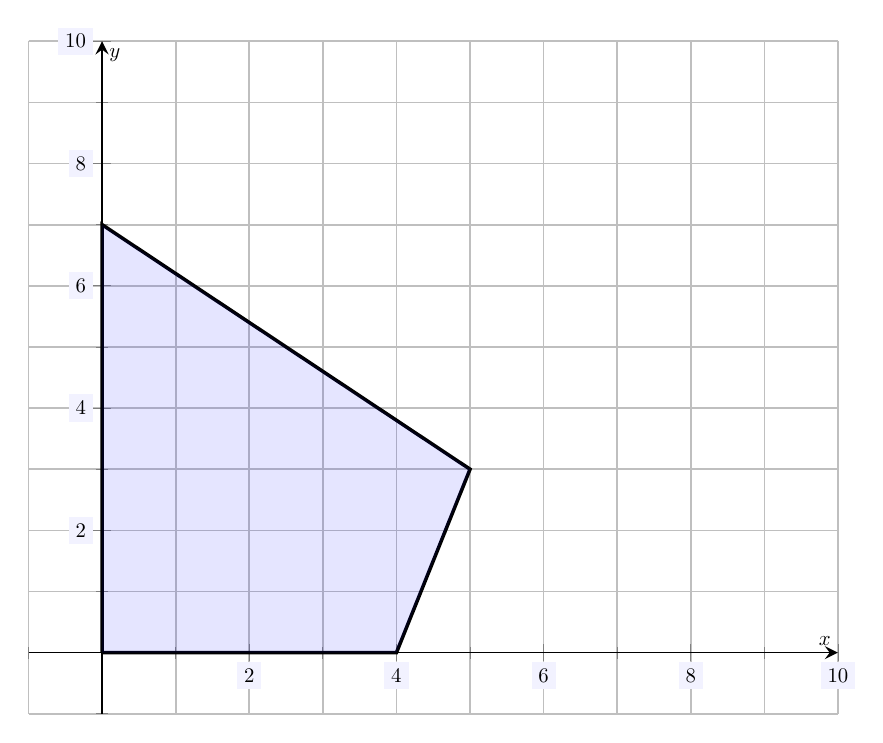
\begin{tikzpicture}[scale=1.5,every node/.style={scale=0.5}]
	\begin{axis}[
	grid=both,
	axis lines=middle,
	ticklabel style={fill=blue!5!white},
	xmin= -1, xmax=10,
	ymin= -1, ymax=10,
	xtick={0,2,4,6,8,10},
	ytick={0,2,4,6,8,10},
	minor tick = {-1,0,1,...,10},
	xlabel=\(x\),ylabel=\(y\),
	]
	\draw[line width=0.03cm] (0,0) -- (0,7) -- (5,3) -- (4,0) -- (0,0);
	\draw[line width=0.01cm,fill= blue,opacity=0.1] (0,0) -- (0,7) -- (5,3) -- (4,0) -- (0,0);
	\end{axis}
	\end{tikzpicture}
	}
	\]



\newpage



% Problem 3
\problem{10} Use the Fundamental of Theorem of Linear Programming to find the maximum and minimum values for the function $f(x, y)$ below given the constraints---also given below.
	\[
	f(x,y)= x + 3y
	\]
	\[
	\left\{
	\begin{aligned}
	x + 5y&\leq 25 \\
	x + y&\leq 9 \\
	-2x + y&\geq -12 \\
	x, y&\geq 0
	\end{aligned} \right.
	\]



\newpage



% Problem 4
\problem{10} Consider the maximization problem given below:
	\[
	\text{max } z= x_1 + 3x_2 - 2x_3
	\]
	\[
	\left\{
	\begin{aligned}
	x_1 + x_2 + x_3&\leq 8 \\
	2x_1 - 3x_2 + x_3&\leq 5 \\
	-x_1 + 4x_2 - 2x_3&\leq 2 \\
	x_1, x_2, x_3&\geq 0
	\end{aligned} \right.
	\]
\begin{enumerate}[(a)]
\item Does the point $(-1, 0, 1)$ satisfy the inequalities above? Explain.
\item Is the point $(2, 3, 1)$ in the feasible region? Explain. 
\item Is the point $(2, 1, 2)$ a feasible point? Explain. If this is a feasible point, find the corresponding $z$ value.
\item Can $(2, 1, 2)$ be a solution to this maximization problem? Explain. [Hint: Can you change some of the variables `a bit' to increase $z$ while still satisfying all the inequalities?]
\end{enumerate}



\newpage



% Problem 5
\problem{10} Write the initial simplex tableau corresponding to the standard maximization problem given below: 
	\[
	\text{max } z= 3x_1 - 4x_2 + x_3
	\]
	\[
	\left\{
	\begin{aligned}
	2x_1 - x_2 &+ 4x_3\leq 8 \\
	x_1 + 6x_3&\leq 5 \\
	x_1, x_2, x_3&\geq 0
	\end{aligned} \right.
	\]



\newpage



% Problem 6
\problem{10} Below is the final simplex tableau corresponding to a standard maximization problem:
	\begin{table}[!ht]
	\centering
	\begin{tabular}{rrrrrrr|r}
	$0$ & $-0.286$ & $0$ & $-0.929$ & $1$ & $-0.071$ & $-0.357$ & $321.0$ \\
	$1$ & $1.07$ & $0$ & $1.36$ & $0$ & $0.143$ & $0.214$ & $607.0$ \\
	$0$ & $0.214$ & $1$ & $0.571$ & $0$ & $-0.071$ & $0.143$ & $71.4$ \\ \hline
	$0$ & $31.8$ & $0$ & $44.3$ & $0$ & $6.38$ & $15.3$ & $35771.43$
	\end{tabular}
	\end{table} 
\begin{enumerate}[(a)]
\item How many inequalities were there for this problem?
\item How many slack variables are present for this problem?
\item How many decision variables were there for this problem?
\item Write the solution to this maximization problem. Your solution should include the maximum values as well as the values for all the decision and slack variables.
\end{enumerate}


\end{document}